% This is "sig-alternate.tex" V2.0 May 2012
% 
\documentclass{sig-alternate}

\usepackage{graphicx}
\usepackage{hyperref}
\usepackage{listings}
\usepackage{multirow}
\usepackage{combelow}
\usepackage{tikz}
\usetikzlibrary{positioning,shapes.geometric,calc}

\lstdefinelanguage{scala}{
  morekeywords={abstract,case,catch,class,def,%
    do,else,extends,false,final,finally,%
    for,if,implicit,import,match,mixin,%
    new,null,object,override,package,%
    private,protected,requires,return,sealed,%
    super,this,throw,trait,true,try,%
    type,val,var,while,with,yield},
  otherkeywords={=>,<-,<\%,<:,>:,\#,@},
  sensitive=true,
  morecomment=[l]{//},
  morecomment=[n]{/*}{*/},
  morestring=[b]",
  morestring=[b]',
  morestring=[b]"""
}
\lstset{breaklines=true, language=scala}

\renewcommand\_{\textunderscore\allowbreak}

\renewcommand{\arraystretch}{1.55}

\begin{document}

\title{ScalaSCA: A Static Bug Finder for Scala\titlenote{Submitted in partial fulfilment of the requirements for CS-498 - Project in Computer Science II, at the Swiss Federal Institute of Technology (EPFL), under the supervision of \textbf{Prof. Viktor Kuncak} (EPFL-LARA) and \textbf{Iulian Drago\cb{s}} (Typesafe Inc.)}}


\numberofauthors{1} 
\author{
\alignauthor
Jean Andr� Gauthier\\
       \affaddr{M.S.c. Computer Science, EPFL}\\
       \email{jean.gauthier@epfl.ch}
}

\makeatletter
\def\@copyrightspace{\relax}
\makeatother

\maketitle
\begin{abstract}
The aim of static code analyses is to detect programming or logic errors before execution, in order to avoid time-consuming code inspection, and most importantly to prevent errors that occur only on a small number of execution paths. Unfortunately, a wide range of those static analyses are computation-intensive, and cannot be included by default as a compiler phase without disrupting the programmer's workflow. In this paper we present \textit{ScalaSCA}, a both fast and extensible static code analysis engine that is implemented as a plugin for the Scala compiler. We discuss some of the bug finding strategies we have implemented and lastly, we measure their performance overhead compared to a standard execution of the Scala compiler.
\end{abstract}

% A category with the (minimum) three required fields
\category{F.3.2.5}{Logics and Meanings of Programs}{Semantics of Programming Languages}[program analysis]

\terms{Verification, Measurement}

\keywords{Static Analysis, Scala, Testing}

\section{Introduction}

In an ideal world, software engineers would be fully reliable and commit no errors at all while developing their software. Since this is obviously not the case, the best they can do is to try to limit the occurrence of such bugs and to standardise the processes of error reporting. This is critical for minimising the amount of time a given bug is left unpatched, and leads to a greater satisfaction of the private or corporate end-users.

As shown in Figure \ref{bugs-table}, the later the stage at which a coding (or design) error is detected, the higher the cost associated to its resolution. Hence, it would make make sense to introduce additional checks at the first machine-level stage, i.e. construction, in order to prevent at least some of the bugs that would usually be detected at later stages of software development. As an example, ``one in a million'' errors that only happen on very few execution paths, but may cause hugh costs when they do occur.

There exist several ways to tackle those issues, each of which has its specific advantages and disadvantages:
\begin{itemize}
\item Manual code review: as developers are notoriously poor at discovering their own bugs, this often implies that two or several developers mutually review their code. But such reviews are often time-consuming (and thus costly), and due to the sheer sizes and complexities of the codebases, very few errors are actually discovered, which leads to a poor cost to bug discovery ratio.
\item Dynamic code analysis: as a first step towards code analysis automation, these analysers\footnote{Cf. \cite{nn07} for the presentation of Valgrind, a collection of dynamic code analysis tools for the C language.} rely on test cases or interactive input during the execution of the target program. Typically, debuggers fall into this category of analysers. While these tools are particularly useful when resolving memory management issues or any dynamic problems involving e.g. reflection, they do not guarantee a complete code coverage with their analysis.
\item Static code analysis: on the other side of the spectrum, static code analysers do not execute the target code at all. This has the consequence that these tools tend to be less suited to the task of solving concurrency or memory issues.\footnote{It should however be noted that this field is an active area of research and there indeed exist techniques that allow a static analysis for potential concurrency issues, as presented in \cite{ww05} for example} Static code analysers are nevertheless an invaluable tool, inasmuch that they usually have a complete code coverage.
\end{itemize}

Ideally, a static code analyser would produce a correctness proof about the code in question. Unfortunately, this is currently infeasible due to the complexity of this task. A more promising approach are correctness proofs about a reduced number of properties, usually specified as assertions. The task of the static analyser is then reduced to proving that the assertion's predicate holds on all execution paths, where relatively good results can be obtained. \footnote{The Leon verification system for Scala is an example of such a tool. \cite{vk13}} A last category of analysers does not try to provide proofs at all but rather flags probable bugs, which is the approach chosen for \textit{ScalaSCA}.

\begin{figure}
\centering
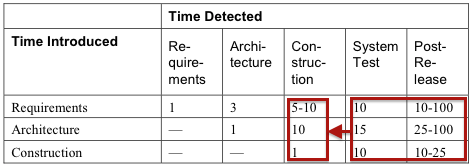
\includegraphics[width=\columnwidth ]{bugs-table.png}
\caption{Cost reduction through bug detection at construction time \cite{smc04}}
\label{bugs-table}
\end{figure}

However, it is important to remember that in practice, code analysis tools are unfortunately frequently measured against the two following metrics, when being integrated in software development cycles:
\begin{itemize}
\item False positives: If the analyser produces too many unnecessary warnings, developers tend to start ignoring them, and this effectively nullifies the purpose of the tool.
\item Execution time: If on the other hand the analyser takes too long to run, it is likely to be taken out of the iterative software development cycle and run too rarely to be helpful in preventing common coding errors.
\end{itemize}
Thus, a static analyser has to strike a balance between performance and accuracy in order to be used in the most effective manner, i.e. during each codebase compilation. This explains why we deliberately oriented the development of \textit{ScalaSCA}'s towards unsound code analyses, in an attempt to improve performance at the expense of making the tool slightly less accurate.

\section{ScalaSCA internals}

\textit{ScalaSCA} has been implemented in order to provide a standardised framework for bug finding strategies. This allows an easier sharing of those strategies across the community, and simplifies the task of programming personalised strategies, if needed.

So-called ``rules'' are the core component of  \textit{ScalaSCA}, as they represent code snippets that perform a specific code analysis. In order to unify the referencing of each one of the rules and allow an easier lookup in bug trackers, a unique identifier has been attributed to each rule, much in the style of \textit{Findbugs} \cite{dwhp04}. \textit{ScalaSCA} differentiates between two types of rules, i.e. rules that can be applied directly on abstract syntax trees (inheriting from the \textbf{ASTRule} class) and general rules (which inherit from \textbf{StandardRule} class).

\subsection{AST Rules}

AST rules impose the following constraints on the developer:
\begin{itemize}
\item A rule name should be specified.
\item The default state, i.e. the state used to initialise the tree-state pair at the first iteration, should be provided.
\item The traversal state and the rule's output should be formalised (by extending \textbf{TraversalState} and \textbf{RuleResult}).
\item A \lstinline{step} method should be defined, taking a tree and a state as arguments and returning a new tree and a new state, to indicate the location where subsequent analyses should be performed. The tree can potentially be missing in order to indicate the end of the traversal.
\item The \lstinline{mergeStates} method should be overridden, in order to specify the information that should be shared between a traversal that has ended, and a still active traversal in the tree-state list. 
\end{itemize}

\textbf{ExampleRule1} summarises these constraints:
\begin{lstlisting}
class ExampleRule1[T <: Global](val global: T, inputResults: List[RuleResult] = List()) extends ASTRule {

 type TS = ...
 type RR = ...

 override val ruleName = ...
 override def getDefaultState(): TS = ...
 
 override def mergeStates(s1: TS, s2: TS): TS = ...
 override def step(tree: Global#Tree, state: TS): List[(Option[TT], TS)] = {
  //... Static analysis of the tree, possibly using results from other rules in inputResults ...
 }
}
\end{lstlisting}

The specification of these methods allows the rules to be traversed in a concurrent fashion by \lstinline{ASTRule.apply()}. Obviously, this only makes sense when a rule is directly working on the AST without using any intermediary representation. Furthermore, if a rule depends on the output of another rule, it will not be possible to run the two analyses concurrently. Instead, the rules should be chained, as explained in Section \ref{sec:practice}.

\subsubsection{Concurrent AST rule traversal}

\textit{ScalaSCA}'s concurrent rule traversal can be invoked by calling the \lstinline{apply} method from the \textbf{ASTRule} object. This method then initialises a map from rules to a list of pairs, consisting of the trees (actually encapsulated in an \textbf{Option}) they have to process next, along with the associated state. Initially, each rule maps to a unique tree (the whole AST) with the state provided by the rule's \lstinline{getDefaultState} method. Then, a call is made to \lstinline{step}, using for each rule the first entry in the tree-state list. This call returns a list of trees and states, according to the locations the analysis should be continued next. If the analysis is stopped for some subtrees, their states are merged together (using the \lstinline{mergeStates} method), and subsequently merged into the state of the next tree to be traversed by the given rule. Once no trees to traverse are left, the final state of each rule's traversal is passed to the rule's \lstinline{getRuleResult} method, and a list of \textbf{RuleResult}s is returned.

\subsection{Standard Rules}

On the other hand, standard rules impose minimalistic contraints on the developer: apart from specifying their name, their only formal requirement is to define the \lstinline{apply} method (specified in the \textbf{StandardRules} abstract class) and to formalise their return type by extending \textbf{RuleResult}:
\begin{lstlisting}
class ExampleRule[T <: Global](val global: T, inputResults: List[RuleResult] = List()) extends StandardRule {
 
 type RR = ...

 override val ruleName = ...
 
 def apply(tree: Tree): RR = {
 //... Static analysis of the tree, possibly using results from other rules in inputResults ...
 }
}
\end{lstlisting}

This freedom, which is necessary for implementing more complex analyses, comes however at a cost: the rule will not be able to participate in the concurrent traversal of the tree. This makes sense in two cases, i.e. when the static analysis is difficult to express in terms of state and position of traversal\footnote{In our experience with \textit{ScalaSCA}, this is usually the case in analyses where the decision on how to continue the analysis depends not only on the current node, but on nodes further down in the tree as well.}, or when the analysis builds up on an intermediary representation.

\subsection{Worklist}

\textit{ScalaSCA} also provides an (experimental) algorithm for solving simple dataflow analyses' equations by computing a fixpoint.

The necessary equations are provided to \textbf{DataflowEquation} in the form of a map from \textbf{ControlFlowGraphNode}s to a function-set pair. The function, which takes \textbf{EquationVaraible}s as input and produces a set of \textbf{ControlFlowGraphNode}s as output, represents the data flow equation for a specific node. The set, second element of the pair, contains the nodes the function is dependent on.

The algorithm itself, based on the worklist algorithm, is implemented in the \textbf{DataflowEquation} class and is run when calling the \lstinline{solve} method on this class:

\begin{lstlisting}[mathescape]
val xArrayBuf = ($\bot$, ... , $\bot$)
val qMList = ($v_1$, ... , $v_n$)
while (!qMList.isEmpty) {
 val $q_i$ = qMList.head
 val y = functionMap($q_i$)(xArrayBuf)
 qMList.remove(0)
 if (y != xArray($q_i$.index)) {
  qMList.append(dependenceMap($q_i$))
  xArray($q_i$.index) = y
 }
}
\end{lstlisting}

While the complexity of this algorithm is quadratic, we sometimes encountered situations where its processing time was slow, and thus decided use a \textbf{Future} to limit the maximal amount of time dedicated to the solving of this equation. Further analyses or improvements of the algorithm can be found e.g. in \cite{ms}.

\section{Example Rules}

Broadly speaking, we envision \textit{ScalaSCA} to be used for the implementation of three categories of rules:
\begin{itemize}
\item Syntactic Rules: these rules work exclusively on ASTs, and do not rely on any intermediate representation.  Rules such as GEN\_BLOCK\_CONST\_PROP or ARI\_DIV\_BY\_ZERO fall into this category. These rules present the advantage that they can be checked in a unique AST traversal, using the \lstinline{ASTRule.apply()} method. It is arguable that this category of rules is the one that captures the best the gist of \textit{ScalaSCA}: simple yet powerful error detection.
\item Intermediate Representation Rules: this category encompasses rules that construct intermediate representations for further analyses, as well as rules that build up upon those representations.

Currently, we have only implemented a control flow graph representation, but the framework could easily be extended with additional intermediate representations, provided they are useful for static analyses.

Dataflow related rules, MEM\_MISSING\_RESOURCE\_CLOSING for example, are a good illustration of rules building up upon such intermediary representations, in our case control flow graphs. They allow to check interesting properties relatively easily, e.g. for sign analyses or variable initialisation, by specifying the necessary equations and lattices.

\item Code metrics: even though we have not implemented any rule measuring code metrics, we deem that this category of rules could provide interesting insights to the developer. These metrics, e.g the lack of cohesion metric (\textit{LCOM}, cf. \cite{hm95}), would probably not be really useful for detecting coding errors. However, they would definitely make sense as quality measurements tools, and could be included in future releases of \textit{ScalaSCA}. 
\end{itemize}

As we have developed several rules for \textit{ScalaSCA}, we briefly present a selection of those:

\subsection{GEN\_BLOCK\_CONST\_PROP}

This rule propagates constants values and stores them in a map. This rule is particularly useful further analyses, e.g. dead code elimination, as the value of of expressions can be computed using this map and the \textbf{ConstantPropagationEvaluator} trait. Table \ref{implementedconstprop} summarises the operations that are currently implemented.

\begin{table*}
\centering
\begin{tabular}{ |c|c| }
\hline
Int & +, -, *, /, \%, <, <=, >, >=, |, \&, $\hat{}$, ==, != \\
Double & +, -, *, /, \%, <, <=, >, >=, ==, != \\
Boolean & \&\&, ||, $\hat{}$, !, ==, != \\
String & +, .length, ==, != \\
List & \\ \hline
\end{tabular}
\caption{Currently implemented operations for constant propagation}
\label{implementedconstprop}
\end{table*}

\subsection{GEN\_CFG\_GENERATOR\_INTRA}

We also have implemented an intraprocedural control flow graph generator in \textit{ScalaSCA}. The analysis takes the conservative approach of ignoring higher order functions, in order to keep the analysis simple. In order to suit the needs of our analyses, we defined several case classes for control flow graph nodes (cf. Table \ref{cfgnodes}). This list will of course be extended if future analyses need a more fine-grained classification of the nodes.

\begin{table*}
\centering
\begin{tabular}{ |c|c| }
\hline
Case class & Used for \\ \hline
MethodDef & Entry point for the control flow graphs \\
ValueDef & Definition of a value  \\
VariableDef & Definition of a variable \\
AssignNode & Assignment \\
ExprNode & Simple expression (currently, anonymous functions also fall into this category)\\
Label & Labels generated for \textbf{while}, \textbf{do ... while} and \textbf{match} constructs \\
MethodCall & Method call on class instances or objects \\
NewNode & Constructor call \\
CatchNode & Parent of all catch cases \\
ThrowNode & \textbf{throw} constructs \\
EmptyNode & Introduced e.g. in the case the \textbf{else} clause is missing\\ \hline
\end{tabular}
\caption{Case classes extending \textbf{ControlFlowGraphNode}}
\label{cfgnodes}
\end{table*}

The analysis starts by introducing a \textbf{MethodDef} node for each analysed method. This node serves as entry point to the graph; no additional nodes are inserted for the exit points, which can be accessed through a list that records the exit nodes of the graph.

In the case of an if-else construct such as
\begin{lstlisting}
A; if (p) { B } else { C }; D
\end{lstlisting}
the generated control flow looks like in Figure \ref{ifelse}. We highlight the fact that in the case of a missing else clause, an \textbf{EmptyNode} is generated instead.

A try-catch-finally construct like
\begin{lstlisting}
A
try { B; C; D }
catch {
 case e: ... => E
 case e: ... => F }
finally { G }
H
\end{lstlisting}
is are processed as shown in Figure \ref{trycatchfinally}. We note the addition of a \textbf{CatchNode}, that groups all incoming exception-related edges. If the \textbf{catch} clause was missing, all edges would be directed to the first \textbf{finally} node. Of course, if the try block was nested inside another try block, the necessary connections between nodes in the inner \textbf{catch} and \textbf{finally} clauses would be drawn to the outer \textbf{catch} clause.

In order to simplify the construction of the control flow graph, we made the assumption that any type of exception could be thrown by any node inside the \textbf{try} clause, and that the partial catch function handles the thrown exception and does not propagate it upwards.

\begin{figure}
\centering
\begin{tikzpicture}[%
    ->,
    shorten >=2pt,
    >=stealth,
    node distance=1cm,
    noname/.style={%
      rectangle,
      minimum width=5em,
      minimum height=3em,
      draw
    }
  ]
    \node[noname] (1) {A};
    \node[noname] (2) [below=of 1] {p: ExprNode};
    \node[noname] (3) [below left=of 2] {B};
    \node[noname] (4) [below right=of 2] {C / EmptyNode};
    \coordinate (Middle) at ($(3)!0.5!(4)$);
    \node[noname] (5) [below=of Middle] {D};

    \path (1) edge node {} (2)
          (2) edge node {} (3)
          (2) edge node {} (4)
          (3) edge node {} (5)
          (4) edge node {} (5);
\end{tikzpicture}
\caption{\textbf{if} ... \textbf{else} ... control flow graph}
\label{ifelse}
\end{figure}


\begin{figure}
\centering
\begin{tikzpicture}[%
    ->,
    shorten >=2pt,
    >=stealth,
    node distance=1cm,
    noname/.style={%
      rectangle,
      minimum width=5em,
      minimum height=3em,
      draw
    }
  ]
    \node[noname] (1) {A};
    \node[noname] (2) [below=of 1] {try: B};
    \node[noname] (3) [below right=of 2] {C};
    \node[noname] (4) [below right=of 3] {D};
    \node[noname] (5) [below left=of 4] {CatchNode};
    \node[noname] (6) [below left=of 5] {case... : E};
    \node[noname] (7) [below right=of 5] {case... : F};
    \coordinate (Middle) at ($(6)!0.5!(7)$);
    \node[noname] (8) [below=of Middle] {G};
    \node[noname] (9) [below=of 8] {H};

    \path (1) edge node {} (2)
          (2) edge node {} (3)
          (2) edge node {} (5)
          (3) edge node {} (4)
          (3) edge node {} (5)
          (4) edge node {} (5)
          (4) edge node {} (8)
          (5) edge node {} (6)
          (5) edge node {} (7)
          (6) edge node {} (8)
          (7) edge node {} (8)
          (8) edge node {} (9);
\end{tikzpicture}
\caption{\textbf{try} ... \textbf{catch} ... \textbf{finally} control flow graph}
\label{trycatchfinally}
\end{figure}

As \textbf{while} and \textbf{match} clauses have already been transformed to labels after the \textit{refchecks} phase, both constructs are handled similarly by the control flow graph generator, i.e. the required edges are being drawn between the label calls and definitions.

\subsection{MEM\_MISSING\_RESOURCE\_CLOSING}

This rule has been implemented very similarly to a reaching definitions dataflow analysis. It builds up upon a control flow graph, that is generated using GEN\_CFG\_GENERATOR\_INTRA. In this analysis, the underlying lattice is
\begin{equation*}
L = 2^{\text{CFGNodes}}
\end{equation*}
where $\text{CFGNodes}$ is the set consisting of all control flow graph nodes. Using this lattice, a system of equations is set up for each node, and the constraints that are used are as follows:
\begin{itemize}
\item For resource opening nodes, the equation
\begin{equation*}
[[\text{node}_\text{open}]] = \left[\bigcup_{n \in \text{pred}(\text{node}_\text{open})}{[[n]]}\right] \cup \{ \text{node}_\text{open} \}
\end{equation*}
is used, with $\text{pred}(n)$ standing for the predecessor nodes of $n$. This can intuitively be explained by the observation that at each node, the set of open resources is the set of resources that were open at the predecessor nodes, plus the current node.
\item Similarly, when a resource is closed, the following equation is used:
\begin{equation*}
[[\text{node}_\text{close}]] = \left[\bigcup_{n \in \text{pred}(\text{node}_\text{close})}{[[n]]}\right] \setminus \{ \text{node}_\text{open} \}
\end{equation*}
\item For all other nodes, the equation is simply:
\begin{equation*}
[[\text{node}]] = \bigcup_{n \in \text{pred}(\text{node}_\text{open})}{[[n]]}
\end{equation*}
\end{itemize}
The solution to this equation system is then computed using \textbf{DataflowEquation}, and if the graph's exit nodes contain unclosed resources, a warning is issued.

It should be noted that this analysis is somewhat imprecise, as it does not detect multiple openings or closings. Furthermore, it is insensitive to situations such as the following one:
\begin{lstlisting}
if (p)
 resource.open()
A
if (p)
 resource.close()
\end{lstlisting}
The reason is that the control flow graph that is generated contains a path where the resource is not closed, as shown on Figure \ref{cfgif} in dashed red. If $p$ was a constant, this could be avoided by running e.g. the dead code elimination rule beforehand, as the if clause would then be removed in any case.

\begin{figure}
\centering
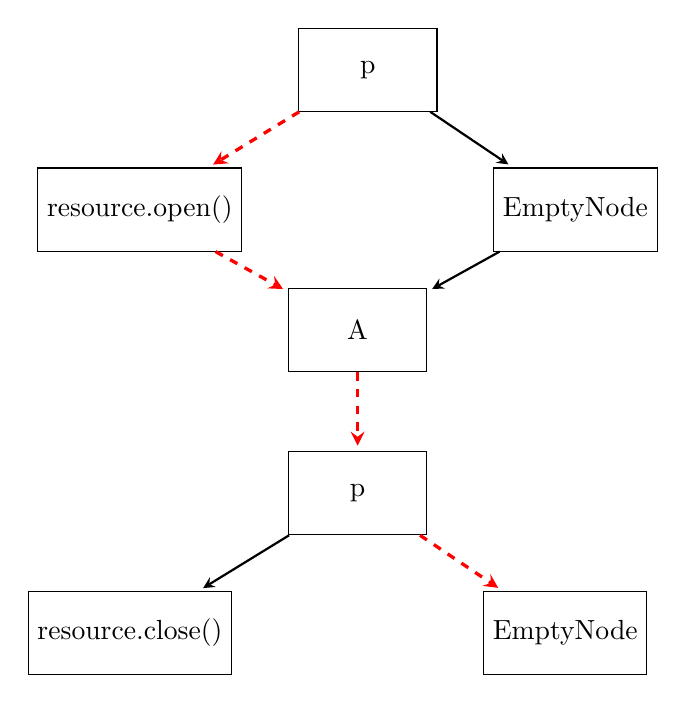
\begin{tikzpicture}[%
    ->,
    shorten >=2pt,
    >=stealth,
    node distance=1cm,
    noname/.style={%
      rectangle,
      minimum width=5em,
      minimum height=3em,
      draw
    }
  ]
    \node[noname] (1) {p};
    \node[noname] (2) [below left=of 1] {resource.open()};
    \node[noname] (3) [below right=of 1] {EmptyNode};
    \coordinate (Middle) at ($(2)!0.5!(3)$);
    \node[noname] (4) [below=of Middle] {A};
    \node[noname] (5) [below=of 4] {p};
    \node[noname] (6) [below left=of 5] {resource.close()};
    \node[noname] (7) [below right=of 5] {EmptyNode};

    \path (1) edge[red,dashed,very thick] node {} (2)
          (1) edge[thick] node {} (3)
          (2) edge[very thick,red,dashed] node {} (4)
          (3) edge[thick] node {} (4)
          (4) edge[very thick,red,dashed] node {} (5)
          (5) edge[thick] node {} (6)
          (5) edge[very thick,red,dashed] node {} (7);
\end{tikzpicture}
\caption{Shortcomings of MEM\_MISSING\_RESOURCE\_CLOSING}
\label{cfgif}
\end{figure}

\section{Implementation}

\textit{ScalaSCA} has been made available free of charge at \url{https://github.com/jean-andre-gauthier/scalasca}, under the 3-clause BSD license. The current implementation is entirely written in Scala, and does not make use of any additional libraries other than the standard Scala library and the Scala compiler library.

As \textit{ScalaSCA} has been developed using the \textit{sbt} interactive build tool, it provides out-of-the-box integration with any existing \textit{sbt} project by simple addition of the following line to any \textit{sbt} project configuration file:
\begin{lstlisting}
addCompilerPlugin("lara.epfl"%%"scalasca"%"0.1")
\end{lstlisting}
This will automatically run the \lstinline{DefaultRule} from \textit{ScalaSCA}. In order to change this behaviour, one or several personalised rules can be set up, compiled to \textit{jar} files and their paths stored line by line in a configuration file. This rules can then be accessed by \textit{ScalaSCA} by specifying the \lstinline{-P:scalasca:c:<config-file-path>} option.

As an example, in an \textit{sbt} configuration file, this option would be specified as follows:
\begin{lstlisting}
scalacOptions <<= (scalacOptions, scalaSource in Compile) {
      (options, base) =>
        options :+ ("-P:scalasca:c:" + configFilePath)
}
\end{lstlisting} 

All compiled rules listed in the configuration file have to define a class named \textbf{ScalaSCAPlugin} with a method \lstinline{createRules} in it. This will allow \textit{ScalaSCA} to invoke this method in order to set up the personalised rules. This plugin mechanism is particularly useful as it allows easily to organise analyses into different categories, e.g. in order to run them at an appropriate time (for example, once a day for slow rules).

For additional details, a sample \textit{ScalaSCA} plugin project has been made available online, at \url{https://github.com/jean-andre-gauthier/scalasca-plugin}.

\section{Performance}

In this section, we present the performance of the tool in practice. We ran \textit{ScalaSCA} on a mid-2013 MacBook Air,\footnote{1.3 GHz Intel Core i5 processor with 8 GB DDR3 Memory} in order to measure the performance on a typical development hardware. We selected four frameworks that cover most sizes of codebases\footnote{Lines of code are not really an indicative measure per se, but are nevertheless a usable as a rough estimate of a codebase's size.}:
\begin{itemize}
\item \textit{ScalaSCA}, our own framework is a relatively small codebase ($\sim$5000 lines of \textit{Scala} code)
\item \textit{Slick}, a database query library developed by \textit{Typesafe Inc.}, contains around 25000 lines of \textit{Scala} code and is a good example of a small to middle sized codebase.
\item \textit{Specs2}, a software specification framework, is a representative example of middle to large sized codebases ($\sim$50000 lines of \textit{Scala} code).
\item \textit{ScalaTest} was the largest codebase we analysed, as it contains more or less 100000 lines of code.
\end{itemize}

All measures have been carried out several times and averaged, in order to produce the values listed in Table \ref{performance}. While this is probably a reasonable way to measure performance, we are well aware that some projects (e.g. \textit{ScalaTest}) are known to interact poorly with certain versions of \textit{Scala}, in terms of compilation performance. As this project explicitly targeted \textit{Scala 2.11}, we used the latest \textit{Scala} version at the time of writing (\textit{2.11.1}) for our measures.

The relative performance was obtained by taking the ratio between the necessary time for a standard compilation and the time taken by a compilation enhanced with \textit{ScalaSCA}. 

Based on our measures, we see that ``syntactic'' rules (i.e. ones using no intermediary representations) do not add a significant overhead to the compilation times. This is also the case for GEN\_CFG\_GENERATOR\_INTRA, which generates a control flow graph and does not add any significant overhead neither. Hence, we deem that these rules could very well be enabled by default and/or integrated to an IDE, due to the minimal variations in terms of performance. On the other hand, rules based on intermediary representations might need to be rethought or optimised before being able to be integrated to an IDE without significantly affecting the workflow.

Interestingly, \textit{ScalaTest} experienced a significant slowdown with \textit{ScalaSCA}, even when being analysed with relatively simple rules. We suppose that this might be due to the way \textit{ScalaTest} was written (i.e. with heavy method overloading), and to the fact that this framework is notoriously memory-intensive for compilation.

We implemented a concurrent traversal of ``syntactic'' rules as we expected a speed up compared to the sequential evaluation of those rules. Unfortunately, as shown by Table \ref{performance2}, there are no significant gains in terms of speed.

Lastly, we note that at the time of writing, an unresolved error occurs when running \textit{ScalaSCA} on \textit{Specs2}. As this error looks relatively similar to other errors we encountered using quasiquotes, we suspect that it might come from the fact that quasiquotes tend to be less stable when applied to ASTs in late compiler phases such as \textit{rechecks}.

\begin{table*}
\centering
\begin{tabular}{ |c|c|c|c|c| }
\hline
 & \textit{ScalaSCA} & \textit{ScalaTest} & \textit{Slick} & \textit{Specs2} \\ \hline
Compilation & 1 & 1 & 1 & 1 \\
ARI\_DIV\_BY\_ZERO & 0.989 & 0.673 & 0.925 & 0.95  \\
GEN\_BLOCK\_CONST\_PROP & 0.99 & 0.644 & 0.864 & ERR \\
GEN\_CFG\_GENERATOR\_INTRA & 0.932 & 0.654 & 0.91 & ERR \\
MEM\_MISSING\_RESOURCE\_CLOSING (experimental) & - & - & - & - \\ \hline
\end{tabular}
\caption{Relative performance of \textit{ScalaSCA} vs. standard compilation}
\label{performance}
\end{table*}

\begin{table*}
\centering
\begin{tabular}{ |c|c|c|c|c| }
\hline
 & \textit{ScalaSCA} & \textit{ScalaTest} & \textit{Slick} & \textit{Specs2} \\ \hline
Compilation & 1 & 1 & 1 & 1 \\
Sequential & 0.725 & 0.54 & 0.87 & 0.94  \\
Concurrent & 0.977 & 0.569 & 0.87 & 0.869 \\ \hline
\end{tabular}
\caption{Relative performance of sequential vs concurrent AST rule evaluation\protect\footnote{Using ARI\_DIV\_BY\_ZERO, BLK\_EMPTY\_FINALLY, MET\_DOUBLE\_TRIPLE\_EQUALS}}
\label{performance2}
\end{table*}

\section{Using ScalaSCA in practice}
\label{sec:practice}

In this section, we present two sample rules of \textit{ScalaSCA}, which allow us to provide more insights into the framework to the reader. The first one is a typical example of a simple ``syntactic'' rule, as it operates directly on ASTs without any need for supplementary information. The second one shows how one could chain two rules in order to use the information computed by the first for improving the precision of the second.

\subsection{Syntactic Rules}
We base our first example on BLK\_EMPTY\_FINALLY, which looks for empty finally blocks, where the developer most likely forgot to include e.g. resource deallocation code.

The first step in defining a new rule is to decide in which format the rule's results should be stored, and in which format potential warnings should be displayed, by extending \textbf{RuleResult} and overriding the three methods \lstinline{warning}, \lstinline{toString} and \lstinline{isSuccess}:
\begin{lstlisting}
case class EmptyFinallyNodes(nodes: List[Global#Position]) extends RuleResult {

 override def warning = Warning("BLK_EMPTY_FINALLY",
  "Empty finally block",
  Console.GREEN + "No empty finally block found" + Console.RESET,
  BadPracticeCategory())

 override def toString: String =
 
  if (nodes.length > 0)
   nodes.foldLeft("")((acc, pos) => acc + "\n" + pos.showError(warning.formattedWarning))
   
  else
   warning.formattedWarning


 override def isSuccess: Boolean =
   nodes.length == 0
}
\end{lstlisting}

The second step consists in creating a case class extending \textbf{TraversalState}, whose instances will store the intermediate results of the traversal:
\begin{lstlisting}
case class EmptyFinallyTraversalState(nodes: List[Global#Position]) extends TraversalState
\end{lstlisting}

Then, the two crucial methods that define the behaviour of the analysis are specified.
\begin{itemize}
\item The first one, \lstinline{step(tree, state)} (1), takes a \lstinline{Tree} and a \lstinline{TraversalState} as parameters. These parameters represent the current location of the traversal and the state of the traversal at that location, respectively. The body of the method specifies where the analysis continues next, and more importantly, whether it corresponds to a faulty pattern, in which case we modify the state by including the current node. Once this detection is done, the method can either spawn new tree and state pairs for a subsequent traversal (by calling \lstinline{goto} or \lstinline{gotoChildren}, possibly specifying a different state for each new position), or decide to stop the traversal if a specific condition (3) is met (by calling \lstinline{gotoLeaf}, of course including the accumulated state).
\item \lstinline{mergeStates(s1, s2)} gets called by the framework when a traverser stops its traversal. In that case, the state of this traverser (\lstinline{s1}) is merged with the state of the next traverser (\lstinline{s2}) in the tree-state list. The second traverser's state is then set to the new state thus obtained.
\end{itemize} 
\begin{lstlisting}
class EF[T <: Global](val global: T, inputResults: List[RuleResult] = List()) extends ASTRule {

 import global._

 type TS = EFTraversalState
 type RR = EFNodes

 override val ruleName = "BLK_EMPTY_FINALLY"

 override def getDefaultState(): TS = EFTraversalState(List())

 override def getRuleResult(state: TS): RR = EFNodes(state.nodes.sortBy(_.pos.point))

(2)override def mergeStates(s1: TS, s2: TS): TS =
   EFTraversalState((s1.nodes ::: s2.nodes).distinct)

(1)override def step(tree: Global#Tree, state: TS): List[(Option[TT], TS)] = tree match {

   case q"try $exprTry catch $cases finally {}" =>
    gotoChildren(tree, state.copy(nodes = tree.pos :: state.nodes))
    
   case q"try $exprTry finally {}" =>
    gotoChildren(tree, state.copy(nodes = tree.pos :: state.nodes))
    
(3)case <<Stop the traversal>> =>
    gotoLeaf(state)
    
   case _ =>
    gotoChildren(tree, state)
 }

 def apply(syntaxTree: Tree): RR = {
  ASTRule.apply(global)(syntaxTree, List(this)) match {
  
   case result :: rest => result match {
    case e @ EFNodes(_) => e
    case _ => EFNodes(List())
   }
   
   case _ => EFNodes(List())
  }
 }
}
\end{lstlisting}

It should be noted that in this simple example, the state simply acted as an accumulator for the locations of the detected errors. The framework however leaves it open to the developer to elaborate more complicated concepts: one could for example store the position of the current node in the state, in order to know at the next step of the traversal which was the previous node of the traversal. Thus, this is a good illustration of the philosophy behind \textit{ScalaSCA}, that purposely avoids imposing too many contraints on the developer, but instead leaves him/her a large degree of freedom when implementing syntactic checks.

\subsection{Chained Rules}
This rule is inspired from a rule we implemented ourselves, i.e. ARI\_DIV\_BY\_ZERO, and shows how the results of static analyses can be shared between different rules. As for the previous rule, we start by extending \textbf{RuleResult}, in order to set up appropriate warning messages:

\begin{lstlisting}
case class DivisionByZeroNodes(nodes: List[Global#Position]) extends RuleResult {
 override def warning = ...
 override def toString: String = ...
 override def isSuccess: Boolean = ...
}
\end{lstlisting}

Secondly, we extend \textbf{TraversalState}, in order to keep track of the necessary information during the traversal.

\begin{lstlisting}
case class DivisionByZeroState(nodes: List[Global#Position]) extends TraversalState
\end{lstlisting}

And lastly, we implement the rule itself, by implementing the \lstinline{mergeStates}, \lstinline{step} and \lstinline{apply} methods :\footnote{for conciseness, division by zero has been abbreviated to DBZ}
\begin{lstlisting}
class DBZ[T <: Global](val global: T, inputResults: List[RuleResult] = List()) extends ASTRule with ConstantPropagationEvaluator {

 //... Usual rule definitions ...

 override def mergeStates(s1: TS, s2: TS): TS =
   DBZState((s1.nodes ::: s2.nodes).distinct)

(1)private val inputSymbolMap = SymbolMapper.getLiteralMapping(inputResults)

 override def step(tree: Global#Tree, state: TS): List[(Option[TT], TS)] = tree match {
 
   //Candidate node for a division by zero
   case Apply(Select(rcvr, TermName("$div")), List(denominator)) if rcvr.tpe <:< typeOf[Int] =>
(2)evaluateToConstant(denominator)(global)(inputSymbolMap) match {

     case Some(value) if value == 0 =>
      gotoLeaf(state.copy(nodes = tree.pos :: state.nodes))
      
     case _ =>
      gotoChildren(List(rcvr, denominator), state)
    }
    
    //Not a division operator
   case _ =>
    gotoChildren(tree, state)
 }

 override def apply(tree: Tree): RR = {
   //... Standard apply method ...
 }
}
\end{lstlisting}

We highlight the fact that with (1), we obtain obtain the mapping between symbols and integers, in this specific case from constant propagation. The types of this mapping are not restricted to the two previous types, as \lstinline{getLiteralMapping} from \lstinline{SymbolMapper} could easily be overloaded to return different kinds of maps, such as maps to sets or intervals for example. In (2), we actually make use of the map and try to evaluate the expression to a constant. If this is possible and the value is equal to 0, we use \lstinline{gotoLeaf} to indicate the end of the traversal of this specific subtree. Otherwise, \lstinline{gotoChildren} analyses the tree root's children.

This example shows that \textit{ScalaSCA} imposes few constraints on the developer, but nonetheless allow to share results of different rules in an intuitive manner, in order to make an analysis more precise.
 
\section{Related work}

Research in static code analysis has been conduced for most programming languages, one of the earliest examples of static checkers being the \textit{lint} checker for the \textit{C} programming language \cite{sj78}. \textit{lint} inspired many code analysis tools, such as \textit{splint} \cite{de02} for example, whose philosophy is to avoid false positives at all costs. Among others, \textit{Goanna} for \textit{C++} \cite{rh08} takes an interesting approach as it is based on a model checker (\textit{NuSMV}) but still manages to show a relatively good performance. Much work has also been dedicated to the \textit{Java} programming language, and various tools have been developed, such as \textit{FindBugs} \cite{dwhp04}, that focuses on simplicity over complexity, or \textit{soot} \cite{vr99} which is a framework that provides intermediate representations of java bytecode. \textit{ScalaSCA} is not the first foray into static analysis on Scala code, and some more complex tools that stay accurate even in the presence of first-class functions are available, e.g. \textit{Insane} \cite{vk14}.

Dynamic programming languages have features which tend to complicate static analyses, as they generally expose less information to the analyser. Previous research has been investigating static analysis for languages such as PHP \cite{vk10} or Javascript \cite{shj09}.

\section{Future work}

In the current form, there are many improvements we envision for\textit{ScalaSCA}: as a first important step, additional rules should be included in the library, in order to improve the usefulness of a \textit{ScalaSCA} run. We also think that providing additional intermediate representations would be beneficial for developers, as this would  prevent the proliferation of independently developed rules that construct those intermediate representations.

A further interesting direction in which \textit{ScalaSCA} could be developed would be the addition of a series of code style checks. Those would allow new as well as more seasoned developers to measure the quality of their code. Lastly, we also think that \textit{ScalaSCA} could be enhanced to provide various code metrics in order to present useful statistics to the developers.

\section{Acknowledgements}

The author wishes to thank his supervisors, Professor Viktor Kuncak and Iulian Drago\cb{s}, for the insightful advice and comments they provided during the development of \textit{ScalaSCA}. In addition, a special thank you to everyone from LARA and Typesafe Inc. who attended our meetings.

\bibliographystyle{abbrv}
\bibliography{paper}

\end{document}
